\documentclass[]{article}
\usepackage{lmodern}
\usepackage{amssymb,amsmath}
\usepackage{ifxetex,ifluatex}
\usepackage{fixltx2e} % provides \textsubscript
\ifnum 0\ifxetex 1\fi\ifluatex 1\fi=0 % if pdftex
  \usepackage[T1]{fontenc}
  \usepackage[utf8]{inputenc}
\else % if luatex or xelatex
  \ifxetex
    \usepackage{mathspec}
  \else
    \usepackage{fontspec}
  \fi
  \defaultfontfeatures{Ligatures=TeX,Scale=MatchLowercase}
\fi
% use upquote if available, for straight quotes in verbatim environments
\IfFileExists{upquote.sty}{\usepackage{upquote}}{}
% use microtype if available
\IfFileExists{microtype.sty}{%
\usepackage{microtype}
\UseMicrotypeSet[protrusion]{basicmath} % disable protrusion for tt fonts
}{}
\usepackage[margin=1in]{geometry}
\usepackage{hyperref}
\hypersetup{unicode=true,
            pdftitle={Trabalho 2 de TGT410029 -- Leg. Territorial e PVG},
            pdfauthor={Willian Zonato; Luiz Fernando Palin Droubi},
            pdfborder={0 0 0},
            breaklinks=true}
\urlstyle{same}  % don't use monospace font for urls
\usepackage{color}
\usepackage{fancyvrb}
\newcommand{\VerbBar}{|}
\newcommand{\VERB}{\Verb[commandchars=\\\{\}]}
\DefineVerbatimEnvironment{Highlighting}{Verbatim}{commandchars=\\\{\}}
% Add ',fontsize=\small' for more characters per line
\usepackage{framed}
\definecolor{shadecolor}{RGB}{248,248,248}
\newenvironment{Shaded}{\begin{snugshade}}{\end{snugshade}}
\newcommand{\KeywordTok}[1]{\textcolor[rgb]{0.13,0.29,0.53}{\textbf{#1}}}
\newcommand{\DataTypeTok}[1]{\textcolor[rgb]{0.13,0.29,0.53}{#1}}
\newcommand{\DecValTok}[1]{\textcolor[rgb]{0.00,0.00,0.81}{#1}}
\newcommand{\BaseNTok}[1]{\textcolor[rgb]{0.00,0.00,0.81}{#1}}
\newcommand{\FloatTok}[1]{\textcolor[rgb]{0.00,0.00,0.81}{#1}}
\newcommand{\ConstantTok}[1]{\textcolor[rgb]{0.00,0.00,0.00}{#1}}
\newcommand{\CharTok}[1]{\textcolor[rgb]{0.31,0.60,0.02}{#1}}
\newcommand{\SpecialCharTok}[1]{\textcolor[rgb]{0.00,0.00,0.00}{#1}}
\newcommand{\StringTok}[1]{\textcolor[rgb]{0.31,0.60,0.02}{#1}}
\newcommand{\VerbatimStringTok}[1]{\textcolor[rgb]{0.31,0.60,0.02}{#1}}
\newcommand{\SpecialStringTok}[1]{\textcolor[rgb]{0.31,0.60,0.02}{#1}}
\newcommand{\ImportTok}[1]{#1}
\newcommand{\CommentTok}[1]{\textcolor[rgb]{0.56,0.35,0.01}{\textit{#1}}}
\newcommand{\DocumentationTok}[1]{\textcolor[rgb]{0.56,0.35,0.01}{\textbf{\textit{#1}}}}
\newcommand{\AnnotationTok}[1]{\textcolor[rgb]{0.56,0.35,0.01}{\textbf{\textit{#1}}}}
\newcommand{\CommentVarTok}[1]{\textcolor[rgb]{0.56,0.35,0.01}{\textbf{\textit{#1}}}}
\newcommand{\OtherTok}[1]{\textcolor[rgb]{0.56,0.35,0.01}{#1}}
\newcommand{\FunctionTok}[1]{\textcolor[rgb]{0.00,0.00,0.00}{#1}}
\newcommand{\VariableTok}[1]{\textcolor[rgb]{0.00,0.00,0.00}{#1}}
\newcommand{\ControlFlowTok}[1]{\textcolor[rgb]{0.13,0.29,0.53}{\textbf{#1}}}
\newcommand{\OperatorTok}[1]{\textcolor[rgb]{0.81,0.36,0.00}{\textbf{#1}}}
\newcommand{\BuiltInTok}[1]{#1}
\newcommand{\ExtensionTok}[1]{#1}
\newcommand{\PreprocessorTok}[1]{\textcolor[rgb]{0.56,0.35,0.01}{\textit{#1}}}
\newcommand{\AttributeTok}[1]{\textcolor[rgb]{0.77,0.63,0.00}{#1}}
\newcommand{\RegionMarkerTok}[1]{#1}
\newcommand{\InformationTok}[1]{\textcolor[rgb]{0.56,0.35,0.01}{\textbf{\textit{#1}}}}
\newcommand{\WarningTok}[1]{\textcolor[rgb]{0.56,0.35,0.01}{\textbf{\textit{#1}}}}
\newcommand{\AlertTok}[1]{\textcolor[rgb]{0.94,0.16,0.16}{#1}}
\newcommand{\ErrorTok}[1]{\textcolor[rgb]{0.64,0.00,0.00}{\textbf{#1}}}
\newcommand{\NormalTok}[1]{#1}
\usepackage{graphicx,grffile}
\makeatletter
\def\maxwidth{\ifdim\Gin@nat@width>\linewidth\linewidth\else\Gin@nat@width\fi}
\def\maxheight{\ifdim\Gin@nat@height>\textheight\textheight\else\Gin@nat@height\fi}
\makeatother
% Scale images if necessary, so that they will not overflow the page
% margins by default, and it is still possible to overwrite the defaults
% using explicit options in \includegraphics[width, height, ...]{}
\setkeys{Gin}{width=\maxwidth,height=\maxheight,keepaspectratio}
\IfFileExists{parskip.sty}{%
\usepackage{parskip}
}{% else
\setlength{\parindent}{0pt}
\setlength{\parskip}{6pt plus 2pt minus 1pt}
}
\setlength{\emergencystretch}{3em}  % prevent overfull lines
\providecommand{\tightlist}{%
  \setlength{\itemsep}{0pt}\setlength{\parskip}{0pt}}
\setcounter{secnumdepth}{5}
% Redefines (sub)paragraphs to behave more like sections
\ifx\paragraph\undefined\else
\let\oldparagraph\paragraph
\renewcommand{\paragraph}[1]{\oldparagraph{#1}\mbox{}}
\fi
\ifx\subparagraph\undefined\else
\let\oldsubparagraph\subparagraph
\renewcommand{\subparagraph}[1]{\oldsubparagraph{#1}\mbox{}}
\fi

%%% Use protect on footnotes to avoid problems with footnotes in titles
\let\rmarkdownfootnote\footnote%
\def\footnote{\protect\rmarkdownfootnote}

%%% Change title format to be more compact
\usepackage{titling}

% Create subtitle command for use in maketitle
\newcommand{\subtitle}[1]{
  \posttitle{
    \begin{center}\large#1\end{center}
    }
}

\setlength{\droptitle}{-2em}

  \title{Trabalho 2 de TGT410029 -- Leg. Territorial e PVG}
    \pretitle{\vspace{\droptitle}\centering\huge}
  \posttitle{\par}
    \author{Willian Zonato \\ Luiz Fernando Palin Droubi}
    \preauthor{\centering\large\emph}
  \postauthor{\par}
      \predate{\centering\large\emph}
  \postdate{\par}
    \date{20 de agosto de 2018}

\usepackage[brazil]{babel}
\usepackage{subfig}
\usepackage{breqn}
\usepackage{booktabs}
\usepackage{longtable}
\usepackage{textcomp}
\usepackage{graphics}
\usepackage{lastpage}
\usepackage{lscape}
\usepackage{indentfirst}
\usepackage[font={it, bf, small}]{caption}
\usepackage{floatrow}
\floatsetup[figure]{capposition=bottom}
\floatsetup[table]{capposition=top}
\usepackage{fancyhdr}
\pagestyle{fancy}
\fancyhf{}
\fancyhead[R]{Página \thepage~de~\pageref{LastPage}}
\newcommand{\pkg}[1]{\textbf{#1}}
\let\proglang=\textsf
\let\code=\texttt
\usepackage{booktabs}
\usepackage{longtable}
\usepackage{array}
\usepackage{multirow}
\usepackage[table]{xcolor}
\usepackage{wrapfig}
\usepackage{float}
\usepackage{colortbl}
\usepackage{pdflscape}
\usepackage{tabu}
\usepackage{threeparttable}
\usepackage{threeparttablex}
\usepackage[normalem]{ulem}
\usepackage{makecell}

\begin{document}
\maketitle

\thispagestyle{empty}

\section{Importação dos dados}\label{importacao-dos-dados}

\begin{enumerate}
\def\labelenumi{\alph{enumi}.}
\tightlist
\item
  Coordenadas
\end{enumerate}

As coordenadas foram extraídas de arquivo .kml\footnote{\url{https://github.com/lfpdroubi/planta_valores/blob/master/Sto_Amaro_4.kml}}
diretamente para o R version 3.5.1 (2018-07-02).

\begin{Shaded}
\begin{Highlighting}[]
\KeywordTok{source}\NormalTok{(}\StringTok{"E:}\CharTok{\textbackslash{}\textbackslash{}}\StringTok{Documents}\CharTok{\textbackslash{}\textbackslash{}}\StringTok{appraiseR}\CharTok{\textbackslash{}\textbackslash{}}\StringTok{R}\CharTok{\textbackslash{}\textbackslash{}}\StringTok{kml.R"}\NormalTok{)}
\NormalTok{df <-}\StringTok{ }\KeywordTok{read.kml}\NormalTok{(}\StringTok{"Sto_Amaro_4.kml"}\NormalTok{, }\StringTok{"Meus lugares"}\NormalTok{)}
\end{Highlighting}
\end{Shaded}

\begin{verbatim}
## OGR data source with driver: KML 
## Source: "E:\Documents\UFSC\Planta de Valores\Trabalho\Sto_Amaro_4.kml", layer: "Meus lugares"
## with 30 features
## It has 2 fields
\end{verbatim}

\rowcolors{2}{gray!6}{white}

\begin{tabular}{lrr}
\hiderowcolors
\toprule
ID & N & E\\
\midrule
\showrowcolors
LT\_01 & -27,68 & -48,76\\
LT\_02 & -27,69 & -48,78\\
LT\_03 & -27,69 & -48,73\\
LT\_04 & -27,68 & -48,76\\
LT\_05 & -27,68 & -48,77\\
LT\_06 & -27,68 & -48,76\\
\bottomrule
\end{tabular}

\rowcolors{2}{white}{white}

\begin{enumerate}
\def\labelenumi{\alph{enumi}.}
\setcounter{enumi}{1}
\tightlist
\item
  Dados do Excel
\end{enumerate}

Os dados da pesquisa de mercado foram lidos diretamente no R version
3.5.1 (2018-07-02).

\begin{Shaded}
\begin{Highlighting}[]
\NormalTok{Dados <-}\StringTok{ }\KeywordTok{read_excel}\NormalTok{(}\StringTok{"Dados.xlsx"}\NormalTok{)}
\end{Highlighting}
\end{Shaded}

\begin{tabular}{lrrrlllll}
\toprule
ID & Area & Valor & VU & Geral & topografia & pavimentacao & pavimentado & situacao\\
\midrule
LT\_01 & 28.750,00 & 3.800.000 & 132,17 & sim & plano & asfalto & sim & esquina\\
LT\_02 & 1.800,00 & 2.700.000 & 1.500,00 & sim & plano & asfalto & sim & meio\\
LT\_03 & 5.373,72 & 250.000 & 46,52 & sim & acidentado & asfalto & sim & meio\\
LT\_04 & 6.188,00 & 880.000 & 142,21 & nao & plano & asfalto & sim & meio\\
LT\_05 & 941,00 & 800.000 & 850,16 & sim & plano & asfalto & sim & meio\\
LT\_06 & 838,72 & 850.000 & 1.013,45 & sim & plano & asfalto & sim & esquina\\
\bottomrule
\end{tabular}

\begin{enumerate}
\def\labelenumi{\alph{enumi}.}
\setcounter{enumi}{2}
\tightlist
\item
  Aglutinação dos dados
\end{enumerate}

Posteriormente, os dados da pesquisa foram mesclados com as coordenadas
dos dados. O conjunto de dados assim obtido pode ser visto na tabela
\ref{tab:geo}

\begin{Shaded}
\begin{Highlighting}[]
\NormalTok{data <-}\StringTok{ }\KeywordTok{inner_join}\NormalTok{(df, Dados, }\DataTypeTok{by =} \StringTok{"ID"}\NormalTok{)}
\end{Highlighting}
\end{Shaded}

\section{Espacialização}\label{espacializacao}

\begin{enumerate}
\def\labelenumi{\alph{enumi}.}
\tightlist
\item
  Criação do conjunto de dados espaciais
\end{enumerate}

Para a transformação dos dados em um conjunto de dados espaciais, basta
informar ao \proglang{R} as colunas das coordenadas e o seu sistema de
referência.

\begin{Shaded}
\begin{Highlighting}[]
\KeywordTok{coordinates}\NormalTok{(data) <-}\StringTok{ }\ErrorTok{~}\NormalTok{E}\OperatorTok{+}\NormalTok{N}
\KeywordTok{proj4string}\NormalTok{(data) <-}\StringTok{ }\KeywordTok{CRS}\NormalTok{(}\StringTok{"+init=epsg:4326"}\NormalTok{) }\CommentTok{# WGS 84}
\end{Highlighting}
\end{Shaded}

\begin{landscape}\begin{table}

\caption{\label{tab:geo}Dados com coordenadas geográficas (WGS-84)}
\centering
\begin{tabular}[t]{lrrrlllllrr}
\toprule
ID & Area & Valor & VU & Geral & topografia & pavimentacao & pavimentado & situacao & E & N\\
\midrule
LT\_01 & 28.750,00 & 3.800.000 & 132,17 & sim & plano & asfalto & sim & esquina & -48,76 & -27,68\\
LT\_02 & 1.800,00 & 2.700.000 & 1.500,00 & sim & plano & asfalto & sim & meio & -48,78 & -27,69\\
LT\_03 & 5.373,72 & 250.000 & 46,52 & sim & acidentado & asfalto & sim & meio & -48,73 & -27,69\\
LT\_04 & 6.188,00 & 880.000 & 142,21 & nao & plano & asfalto & sim & meio & -48,76 & -27,68\\
LT\_05 & 941,00 & 800.000 & 850,16 & sim & plano & asfalto & sim & meio & -48,77 & -27,68\\
\addlinespace
LT\_06 & 838,72 & 850.000 & 1.013,45 & sim & plano & asfalto & sim & esquina & -48,76 & -27,68\\
LT\_07 & 777,00 & 690.000 & 888,03 & sim & plano & asfalto & sim & meio & -48,75 & -27,68\\
LT\_08 & 630,00 & 600.000 & 952,38 & sim & plano & blokret & sim & esquina & -48,75 & -27,68\\
LT\_09 & 1.740,00 & 380.000 & 218,39 & nao & plano & blokret & sim & meio & -48,78 & -27,69\\
LT\_12 & 585,00 & 240.000 & 410,26 & nao & plano & asfalto & sim & esquina & -48,78 & -27,68\\
\addlinespace
LT\_13 & 668,29 & 230.000 & 344,16 & nao & plano & blokret & sim & meio & -48,75 & -27,68\\
LT\_16 & 700,00 & 150.000 & 214,29 & nao & acidentado & blokret & sim & meio & -48,78 & -27,69\\
LT\_17 & 360,00 & 130.000 & 361,11 & nao & plano & blokret & sim & meio & -48,76 & -27,68\\
LT\_22 & 385,00 & 95.000 & 246,75 & nao & acidentado & blokret & sim & meio & -48,75 & -27,71\\
LT\_26 & 472,00 & 380.000 & 805,08 & sim & plano & asfalto & sim & meio & -48,76 & -27,68\\
\addlinespace
LT\_27 & 380,00 & 285.000 & 750,00 & nao & plano & blokret & sim & meio & -48,78 & -27,69\\
LT\_29 & 2.261,00 & 398.000 & 176,03 & nao & plano & asfalto & sim & meio & -48,73 & -27,69\\
LT\_30 & 30.000,00 & 850.000 & 28,33 & nao & plano & asfalto & sim & meio & -48,77 & -27,68\\
LT\_31 & 360,00 & 180.000 & 500,00 & nao & plano & asfalto & sim & meio & -48,75 & -27,68\\
LT\_32 & 384,00 & 95.000 & 247,40 & nao & acidentado & blokret & sim & meio & -48,77 & -27,68\\
\addlinespace
LT\_33 & 2.000,00 & 2.000.000 & 1.000,00 & nao & plano & blokret & sim & meio & -48,78 & -27,68\\
LT\_35 & 360,00 & 105.000 & 291,67 & nao & plano & blokret & sim & esquina & -48,74 & -27,68\\
LT\_36 & 400,00 & 380.000 & 950,00 & sim & plano & asfalto & sim & esquina & -48,80 & -27,70\\
LT\_37 & 1.507,17 & 420.000 & 278,67 & nao & plano & sem & nao & meio & -48,76 & -27,68\\
LT\_38 & 808,92 & 370.000 & 457,40 & nao & acidentado & asfalto & sim & esquina & -48,78 & -27,69\\
\addlinespace
AVAL\_1 & 360,00 & NA & NA & sim & plano & NA & NA & NA & -48,78 & -27,69\\
AVAL\_2 & 360,00 & NA & NA & sim & acidentado & NA & NA & NA & -48,78 & -27,69\\
AVAL\_3 & 360,00 & NA & NA & nao & acidentado & NA & NA & NA & -48,78 & -27,69\\
AVAL\_4 & 360,00 & NA & NA & nao & plano & NA & NA & NA & -48,78 & -27,69\\
\bottomrule
\end{tabular}
\end{table}
\end{landscape}

\begin{enumerate}
\def\labelenumi{\alph{enumi}.}
\setcounter{enumi}{1}
\tightlist
\item
  Escrita do Shapefile no disco
\end{enumerate}

Foi escrito um \emph{shapefile} no disco à partir do conjunto de dados
espaciais, através da função \code{writeOGR}, do pacote \pkg{rgdal}.

\begin{Shaded}
\begin{Highlighting}[]
\CommentTok{# Para escrever o shapefile no disco:  }
 \KeywordTok{writeOGR}\NormalTok{(data, }
          \DataTypeTok{dsn =} \StringTok{"E:}\CharTok{\textbackslash{}\textbackslash{}}\StringTok{Documents}\CharTok{\textbackslash{}\textbackslash{}}\StringTok{UFSC}\CharTok{\textbackslash{}\textbackslash{}}\StringTok{Planta de Valores}\CharTok{\textbackslash{}\textbackslash{}}\StringTok{Trabalho"}\NormalTok{, }
          \DataTypeTok{layer =} \StringTok{"dados"}\NormalTok{,}
          \DataTypeTok{driver =} \StringTok{"ESRI Shapefile"}\NormalTok{,}
          \DataTypeTok{overwrite_layer =} \OtherTok{TRUE}\NormalTok{,}
          \DataTypeTok{delete_dsn =} \OtherTok{TRUE}\NormalTok{)}
\end{Highlighting}
\end{Shaded}

\begin{enumerate}
\def\labelenumi{\alph{enumi}.}
\setcounter{enumi}{2}
\tightlist
\item
  Conversão de unidades
\end{enumerate}

O sistema de referência pode ser alterado através da função
\code{spTransform}, do pacote \pkg{sp}. Por exemplo, para alterar para
SIRGAS2000, basta informar o código EPSG deste sistema de referência
(31997). Os dados com as coordenadas transformadas podem ser vistos na
tabela \ref{tab:SIRGAS}.

\begin{Shaded}
\begin{Highlighting}[]
\CommentTok{# Conversão de coordenadas para SIRGAS2000}
\NormalTok{CRS.new <-}\StringTok{ }\KeywordTok{CRS}\NormalTok{(}\StringTok{"+init=epsg:31997"}\NormalTok{)}
\end{Highlighting}
\end{Shaded}

\begin{landscape}\begin{table}

\caption{\label{tab:SIRGAS}Dados com coordenadas em SIRGAS2000}
\centering
\begin{tabu} to \linewidth {>{\raggedright}X>{\raggedleft}X>{\raggedleft}X>{\raggedleft}X>{\raggedright}X>{\raggedright}X>{\raggedright}X>{\raggedright}X>{\raggedright}X>{\raggedleft}X>{\raggedleft}X}
\toprule
ID & Area & Valor & VU & Geral & topografia & pavimentacao & pavimentado & situacao & E & N\\
\midrule
LT\_01 & 28.750 & 3.800.000 & 132 & sim & plano & asfalto & sim & esquina & 721.057 & 6.935.883\\
LT\_02 & 1.800 & 2.700.000 & 1.500 & sim & plano & asfalto & sim & meio & 719.145 & 6.935.146\\
LT\_03 & 5.374 & 250.000 & 47 & sim & acidentado & asfalto & sim & meio & 724.179 & 6.935.262\\
LT\_04 & 6.188 & 880.000 & 142 & nao & plano & asfalto & sim & meio & 721.200 & 6.936.007\\
LT\_05 & 941 & 800.000 & 850 & sim & plano & asfalto & sim & meio & 719.747 & 6.935.745\\
\addlinespace
LT\_06 & 839 & 850.000 & 1.013 & sim & plano & asfalto & sim & esquina & 720.794 & 6.935.826\\
LT\_07 & 777 & 690.000 & 888 & sim & plano & asfalto & sim & meio & 721.566 & 6.936.011\\
LT\_08 & 630 & 600.000 & 952 & sim & plano & blokret & sim & esquina & 721.423 & 6.936.059\\
LT\_09 & 1.740 & 380.000 & 218 & nao & plano & blokret & sim & meio & 718.600 & 6.935.355\\
LT\_12 & 585 & 240.000 & 410 & nao & plano & asfalto & sim & esquina & 719.123 & 6.936.329\\
\addlinespace
LT\_13 & 668 & 230.000 & 344 & nao & plano & blokret & sim & meio & 721.496 & 6.936.081\\
LT\_16 & 700 & 150.000 & 214 & nao & acidentado & blokret & sim & meio & 718.823 & 6.935.234\\
LT\_17 & 360 & 130.000 & 361 & nao & plano & blokret & sim & meio & 721.383 & 6.936.302\\
LT\_22 & 385 & 95.000 & 247 & nao & acidentado & blokret & sim & meio & 722.114 & 6.932.789\\
LT\_26 & 472 & 380.000 & 805 & sim & plano & asfalto & sim & meio & 721.370 & 6.936.080\\
\addlinespace
LT\_27 & 380 & 285.000 & 750 & nao & plano & blokret & sim & meio & 718.846 & 6.935.437\\
LT\_29 & 2.261 & 398.000 & 176 & nao & plano & asfalto & sim & meio & 723.612 & 6.934.793\\
LT\_30 & 30.000 & 850.000 & 28 & nao & plano & asfalto & sim & meio & 719.513 & 6.936.004\\
LT\_31 & 360 & 180.000 & 500 & nao & plano & asfalto & sim & meio & 721.938 & 6.935.865\\
LT\_32 & 384 & 95.000 & 247 & nao & acidentado & blokret & sim & meio & 719.942 & 6.936.207\\
\addlinespace
LT\_33 & 2.000 & 2.000.000 & 1.000 & nao & plano & blokret & sim & meio & 718.821 & 6.935.955\\
LT\_35 & 360 & 105.000 & 292 & nao & plano & blokret & sim & esquina & 722.757 & 6.936.153\\
LT\_36 & 400 & 380.000 & 950 & sim & plano & asfalto & sim & esquina & 716.888 & 6.933.926\\
LT\_37 & 1.507 & 420.000 & 279 & nao & plano & sem & nao & meio & 721.221 & 6.936.674\\
LT\_38 & 809 & 370.000 & 457 & nao & acidentado & asfalto & sim & esquina & 718.864 & 6.935.252\\
\addlinespace
AVAL\_1 & 360 & NA & NA & sim & plano & NA & NA & NA & 719.186 & 6.935.292\\
AVAL\_2 & 360 & NA & NA & sim & acidentado & NA & NA & NA & 719.186 & 6.935.291\\
AVAL\_3 & 360 & NA & NA & nao & acidentado & NA & NA & NA & 719.185 & 6.935.291\\
AVAL\_4 & 360 & NA & NA & nao & plano & NA & NA & NA & 719.185 & 6.935.291\\
\bottomrule
\end{tabu}
\end{table}
\end{landscape}

\section{Confecção de mapas
temáticos}\label{confeccao-de-mapas-tematicos}

Foram elaborados mapas temáticos de algumas variáveis pesquisadas,
também com o auxílio do \proglang{R}. Nas figuras abaixo, o tamanho dos
pontos foi escalonada de acordo com a escala de valor unitário para cada
dado.

\begin{enumerate}
\def\labelenumi{\alph{enumi}.}
\tightlist
\item
  Topografia
\end{enumerate}

Os terrenos foram classificados em plano (vermelho) e acidentado (azul),
conforme pode ser visto na figura abaixo:

\begin{center}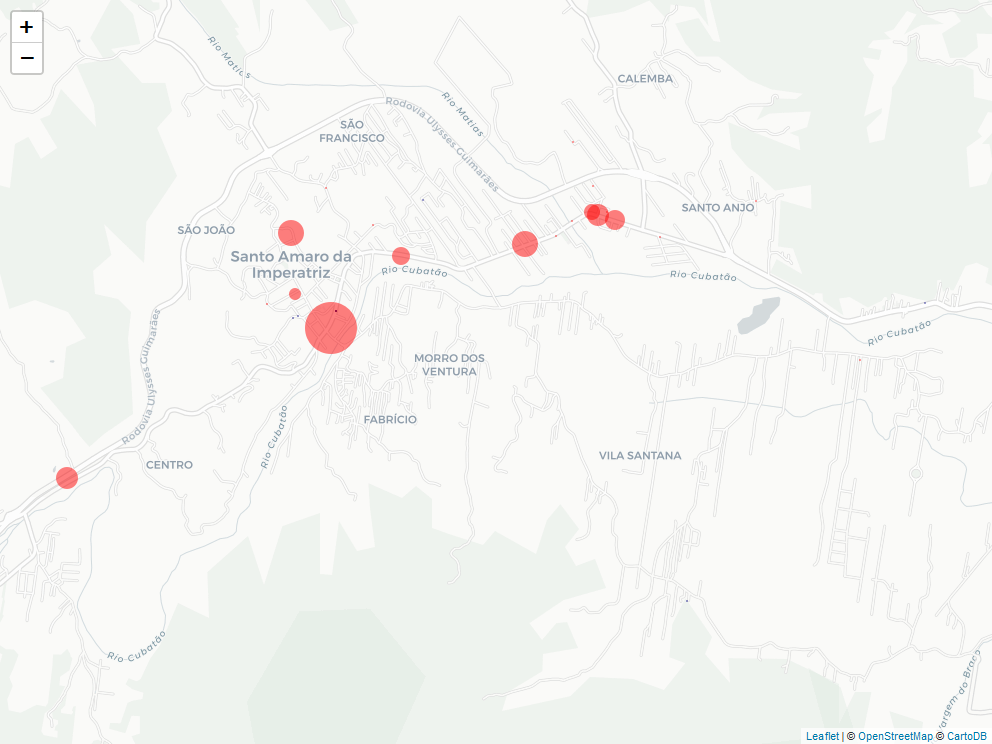
\includegraphics[width=0.5\linewidth]{Report_files/figure-latex/mapa1-1} \end{center}

\begin{enumerate}
\def\labelenumi{\alph{enumi}.}
\setcounter{enumi}{1}
\tightlist
\item
  Pavimentação
\end{enumerate}

Na figura abaixo, os dados podem ser vistos em função da pavimentação da
frente do lote, se asfalto (azul), \emph{blokret} (verde) e sem
pavimentação (vermelho).

\begin{center}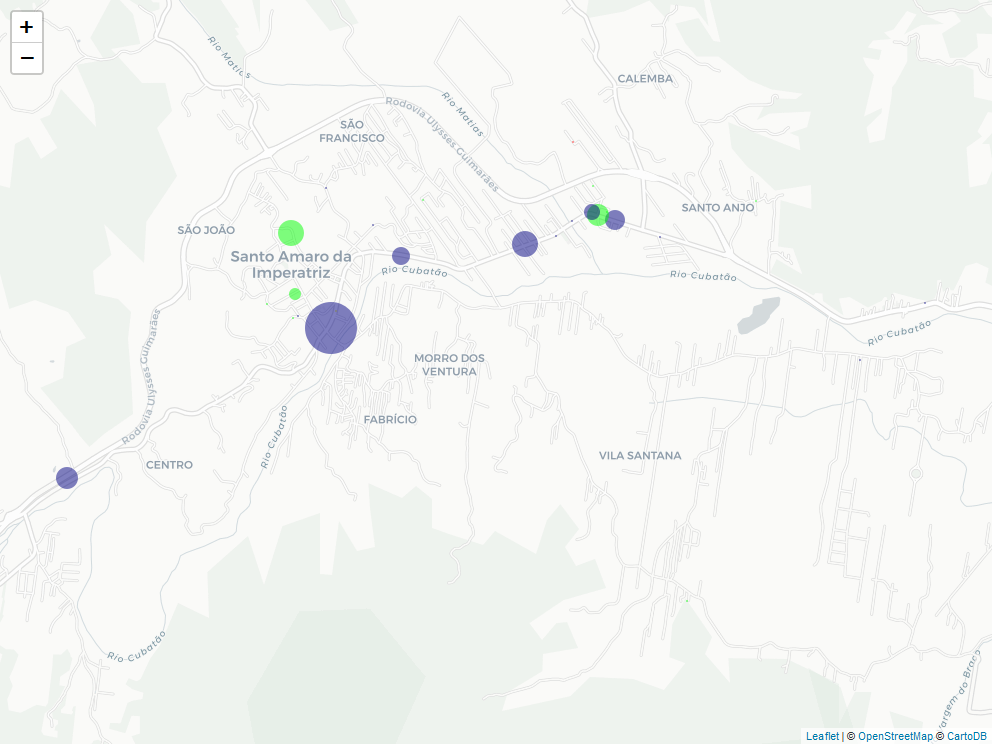
\includegraphics[width=0.5\linewidth]{Report_files/figure-latex/mapa2-1} \end{center}

\begin{enumerate}
\def\labelenumi{\alph{enumi}.}
\setcounter{enumi}{2}
\tightlist
\item
  Situação
\end{enumerate}

Na figura abaixo, os dados de meio de quadra são vistos em azul e os
dados de esquina em vermelho.

\begin{center}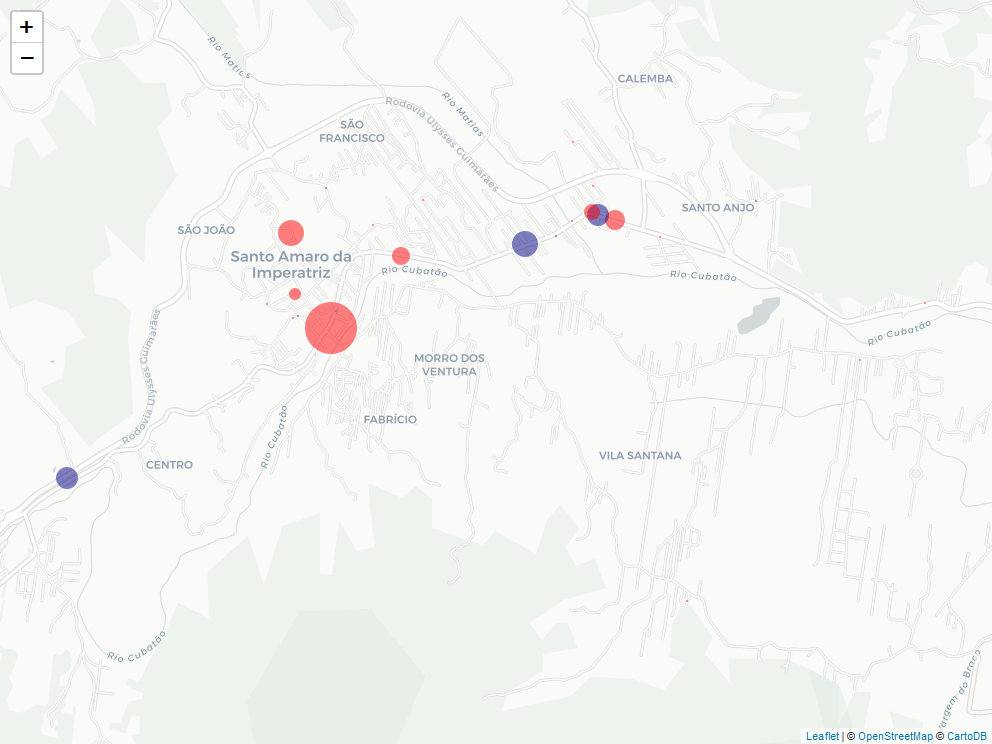
\includegraphics[width=0.5\linewidth]{Report_files/figure-latex/mapa3-1} \end{center}

\section{Ajuste do modelo OLS}\label{ajuste-do-modelo-ols}

Foi ajustado inicialmente um modelo linear com todas as variáveis
pesquisadas:

\begin{Shaded}
\begin{Highlighting}[]
\NormalTok{fit <-}\StringTok{ }\KeywordTok{lm}\NormalTok{(VU }\OperatorTok{~}\StringTok{ }\NormalTok{Area }\OperatorTok{+}\StringTok{ }\NormalTok{Geral }\OperatorTok{+}\StringTok{ }\NormalTok{topografia }\OperatorTok{+}\StringTok{ }\NormalTok{pavimentado }\OperatorTok{+}\StringTok{ }\NormalTok{situacao, }\DataTypeTok{data =}\NormalTok{ data)}
\end{Highlighting}
\end{Shaded}

\section{Diagrama de Box-Cox}\label{diagrama-de-box-cox}

De posse do modelo linear, foi feito o diagrama de Box-Cox, para
pesquisar melhores transformações para a variável dependente.

\begin{center}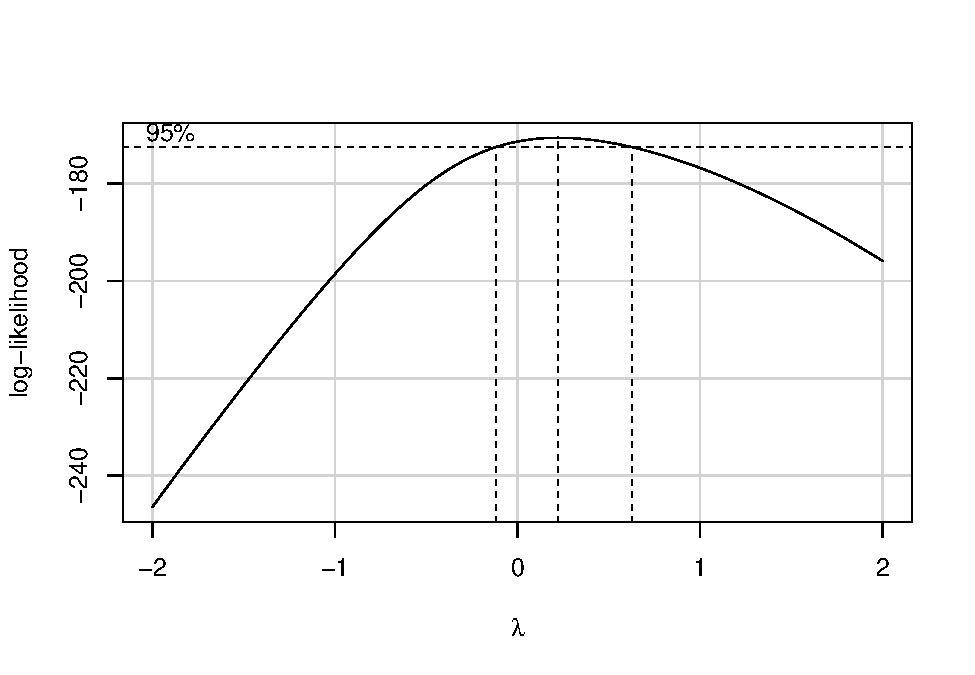
\includegraphics[width=0.7\linewidth]{Report_files/figure-latex/unnamed-chunk-5-1} \end{center}

\section{Modelo final}\label{modelo-final}

Após efetuadas as transformações necessárias, removidos os
\emph{outliers} e as variáveis insignificantes, chegou-se ao modelo
descrito na tabela \ref{tab:fit}.

\begin{table}[!htbp] \centering 
  \caption{Coeficientes do modelo final} 
  \label{tab:fit} 
\begin{tabular}{@{\extracolsep{5pt}}lc} 
\\[-1.8ex]\hline 
\hline \\[-1.8ex] 
 & \multicolumn{1}{c}{\textit{Dependent variable:}} \\ 
\cline{2-2} 
\\[-1.8ex] & log(VU) \\ 
\hline \\[-1.8ex] 
 log(Area) & $-$0.508 ($-$0.637, $-$0.380) \\ 
  & t = $-$7.733 \\ 
  & p = 0.00000$^{***}$ \\ 
  Geralsim & 1.101 (0.753, 1.448) \\ 
  & t = 6.201 \\ 
  & p = 0.00001$^{***}$ \\ 
  topografiaplano & 0.303 ($-$0.146, 0.753) \\ 
  & t = 1.324 \\ 
  & p = 0.202 \\ 
  Constant & 8.825 (7.932, 9.717) \\ 
  & t = 19.380 \\ 
  & p = 0.000$^{***}$ \\ 
 \hline \\[-1.8ex] 
Observations & 23 \\ 
R$^{2}$ & 0.843 \\ 
Adjusted R$^{2}$ & 0.818 \\ 
Residual Std. Error & 0.382 (df = 19) \\ 
F Statistic & 33.962$^{***}$ (df = 3; 19) \\ 
\hline 
\hline \\[-1.8ex] 
\textit{Note:}  & \multicolumn{1}{r}{$^{*}$p$<$0.1; $^{**}$p$<$0.05; $^{***}$p$<$0.01} \\ 
\end{tabular} 
\end{table}

\subsection{Diagnóstico básico}\label{diagnostico-basico}

\begin{figure}[H]

{\centering 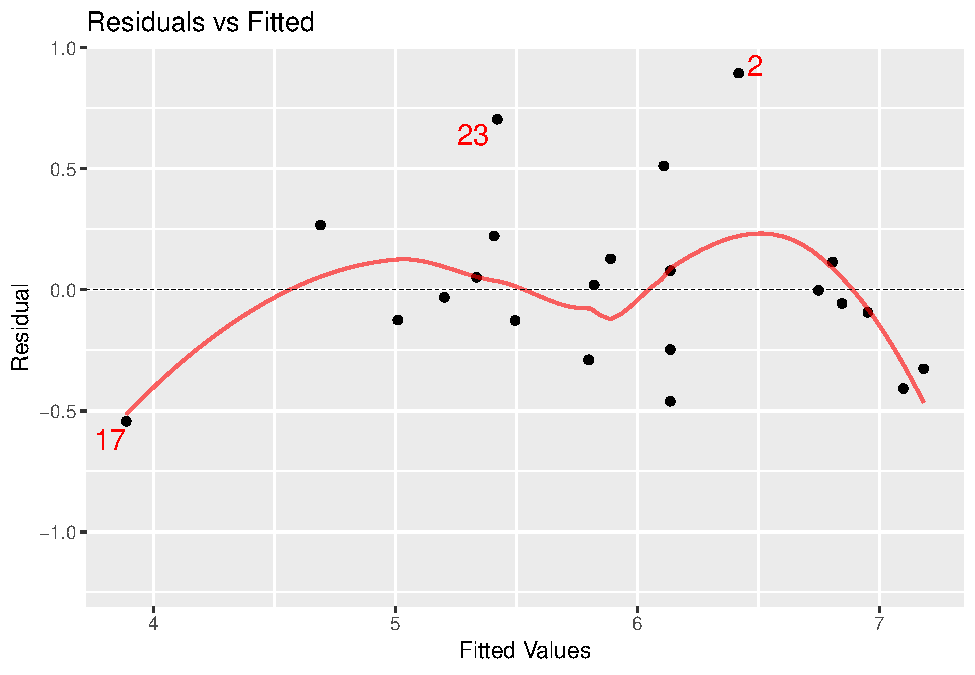
\includegraphics[width=0.34\linewidth]{Report_files/figure-latex/plotfit-1} 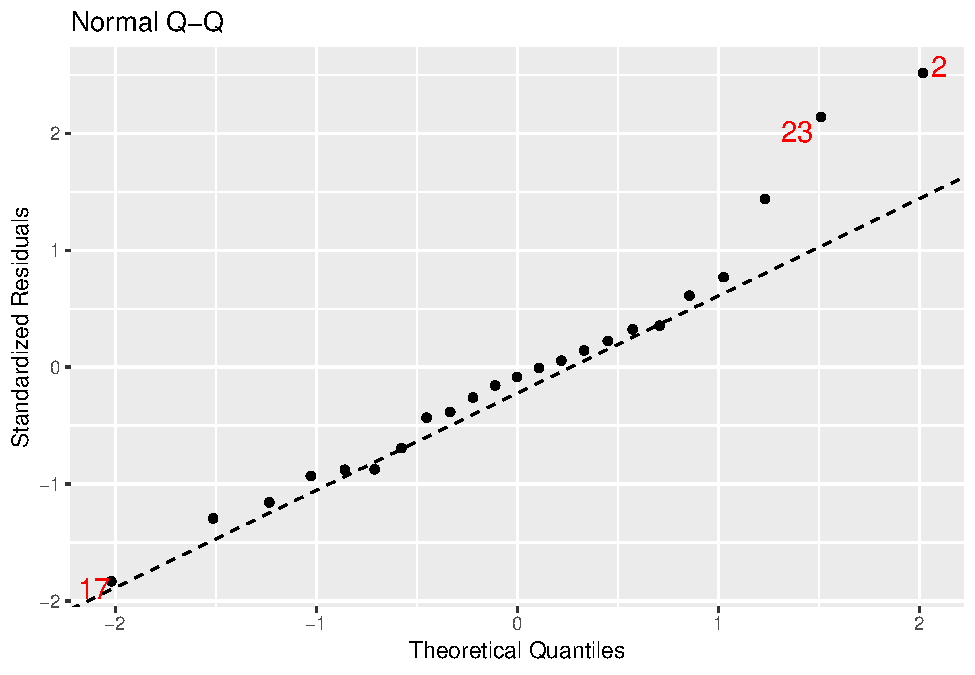
\includegraphics[width=0.34\linewidth]{Report_files/figure-latex/plotfit-2} 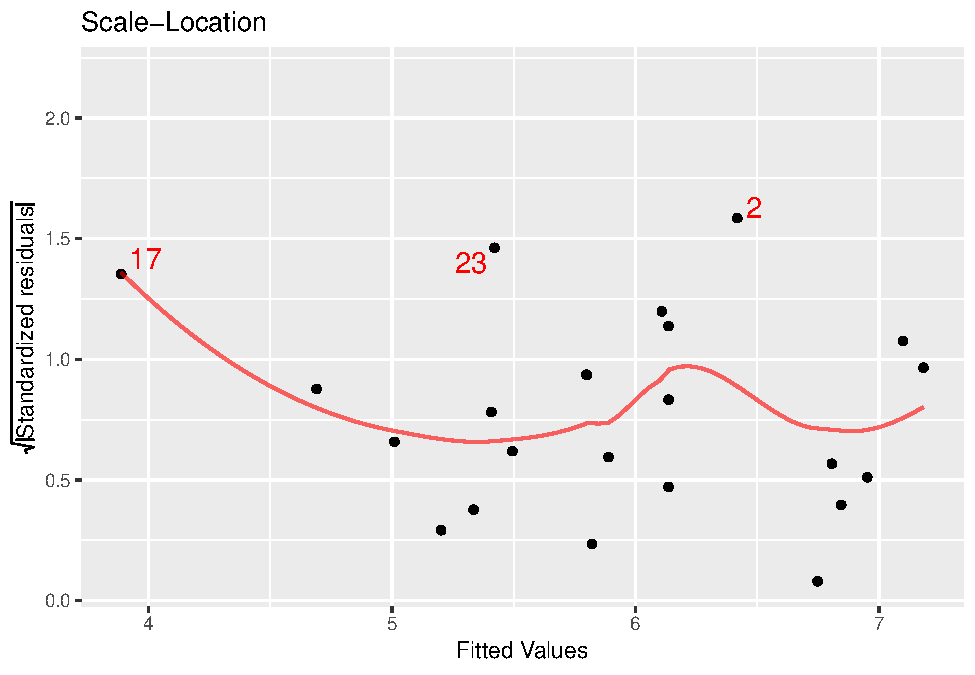
\includegraphics[width=0.34\linewidth]{Report_files/figure-latex/plotfit-3} 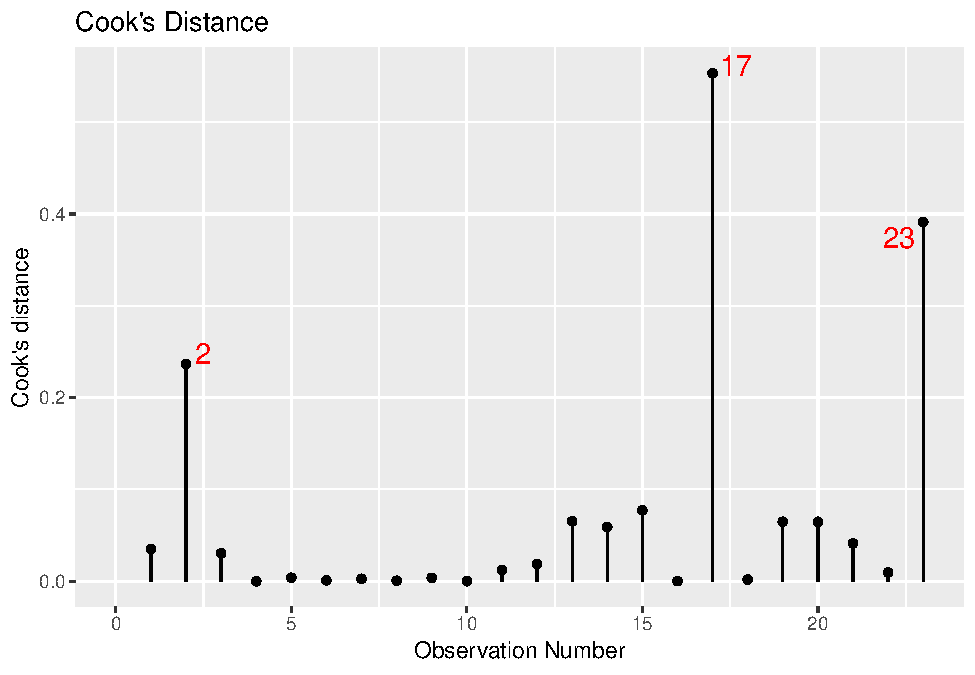
\includegraphics[width=0.34\linewidth]{Report_files/figure-latex/plotfit-4} 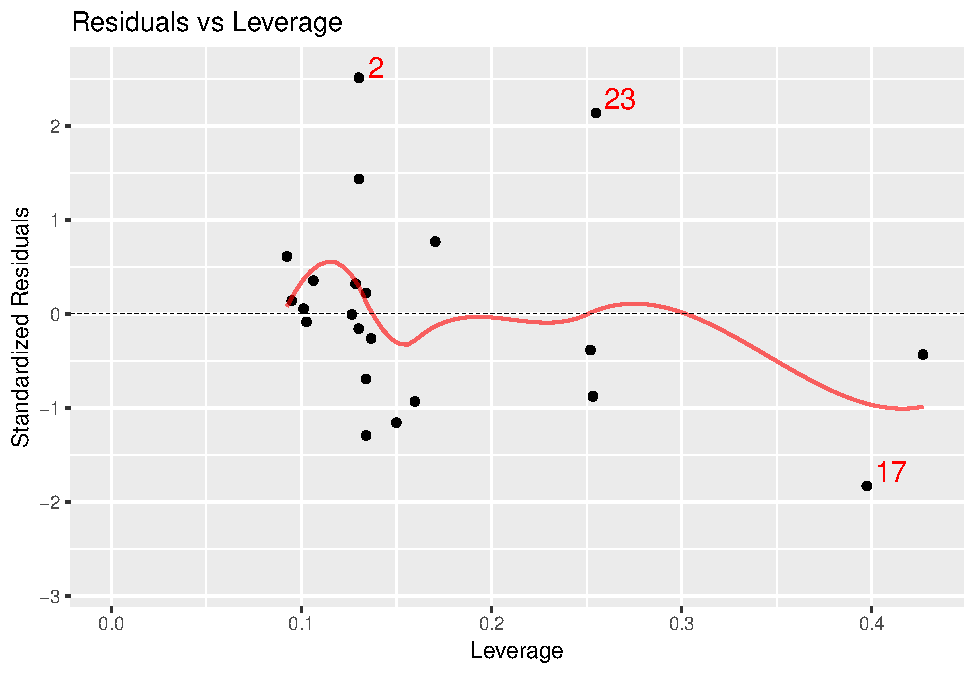
\includegraphics[width=0.34\linewidth]{Report_files/figure-latex/plotfit-5} 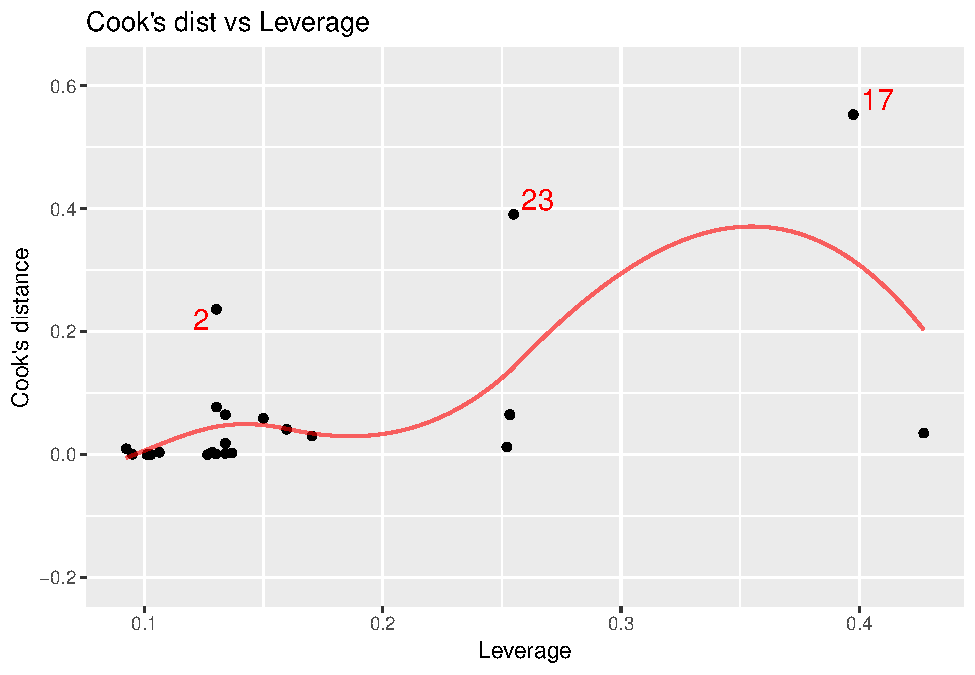
\includegraphics[width=0.34\linewidth]{Report_files/figure-latex/plotfit-6} 

}

\caption{Gráficos básicos do modelo}\label{fig:plotfit}
\end{figure}

\subsection{Testes do modelo}\label{testes-do-modelo}

\subsubsection{Homoscedasticidade}\label{homoscedasticidade}

\begin{verbatim}
## 
##  studentized Breusch-Pagan test
## 
## data:  fit
## BP = 1.0575801, df = 3, p-value = 0.787323
\end{verbatim}

\subsubsection{Normalidade}\label{normalidade}

\begin{enumerate}
\def\labelenumi{\alph{enumi}.}
\tightlist
\item
  Teste de Pearson (\(\chi^2\))
\end{enumerate}

\begin{verbatim}
## 
##  Pearson chi-square normality test
## 
## data:  resid(fit)
## P = 3.7826087, p-value = 0.58112
\end{verbatim}

\begin{enumerate}
\def\labelenumi{\alph{enumi}.}
\setcounter{enumi}{1}
\tightlist
\item
  Teste de Lilliefors (Kolgomorov-Smirnov):
\end{enumerate}

\begin{verbatim}
## 
##  Lilliefors (Kolmogorov-Smirnov) normality test
## 
## data:  resid(fit)
## D = 0.14183288, p-value = 0.2683846
\end{verbatim}

\begin{enumerate}
\def\labelenumi{\alph{enumi}.}
\setcounter{enumi}{2}
\tightlist
\item
  Teste de Shapiro-Wilk:
\end{enumerate}

\begin{verbatim}
## 
##  Shapiro-Wilk normality test
## 
## data:  resid(fit)
## W = 0.94114636, p-value = 0.1901815
\end{verbatim}

\begin{enumerate}
\def\labelenumi{\alph{enumi}.}
\setcounter{enumi}{3}
\tightlist
\item
  Teste de Anderson-Darling:
\end{enumerate}

\begin{verbatim}
## 
##  Anderson-Darling normality test
## 
## data:  resid(fit)
## A = 0.45939696, p-value = 0.2384414
\end{verbatim}

\begin{enumerate}
\def\labelenumi{\alph{enumi}.}
\setcounter{enumi}{4}
\tightlist
\item
  Teste de Jarque-Bera:
\end{enumerate}

\begin{verbatim}
## 
##  Jarque-Bera test for normality
## 
## data:  resid(fit)
## JB = 2.9044081, p-value = 0.089
\end{verbatim}

\newpage

\begin{enumerate}
\def\labelenumi{\alph{enumi}.}
\setcounter{enumi}{5}
\tightlist
\item
  Histograma
\end{enumerate}

\begin{figure}[H]

{\centering 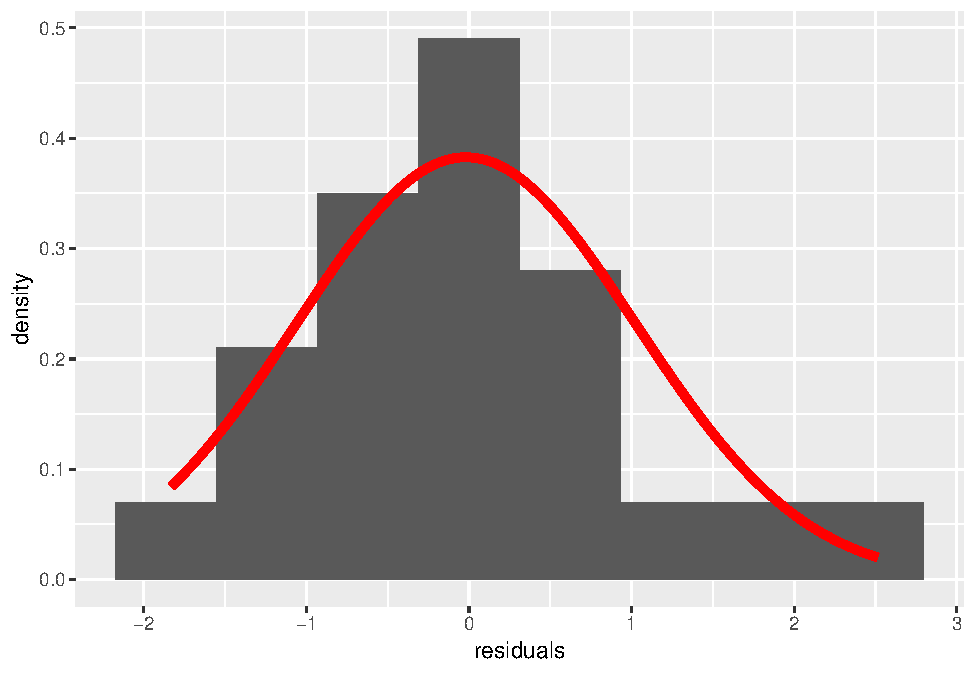
\includegraphics[width=0.45\linewidth]{Report_files/figure-latex/histograma-1} 

}

\caption{Histograma dos resíduos padronizados}\label{fig:histograma}
\end{figure}

\begin{enumerate}
\def\labelenumi{\alph{enumi}.}
\setcounter{enumi}{6}
\tightlist
\item
  Teste K-S (Kolgomorov-Smirnov) {[}@KS{]}
\end{enumerate}

\begin{figure}[H]

{\centering 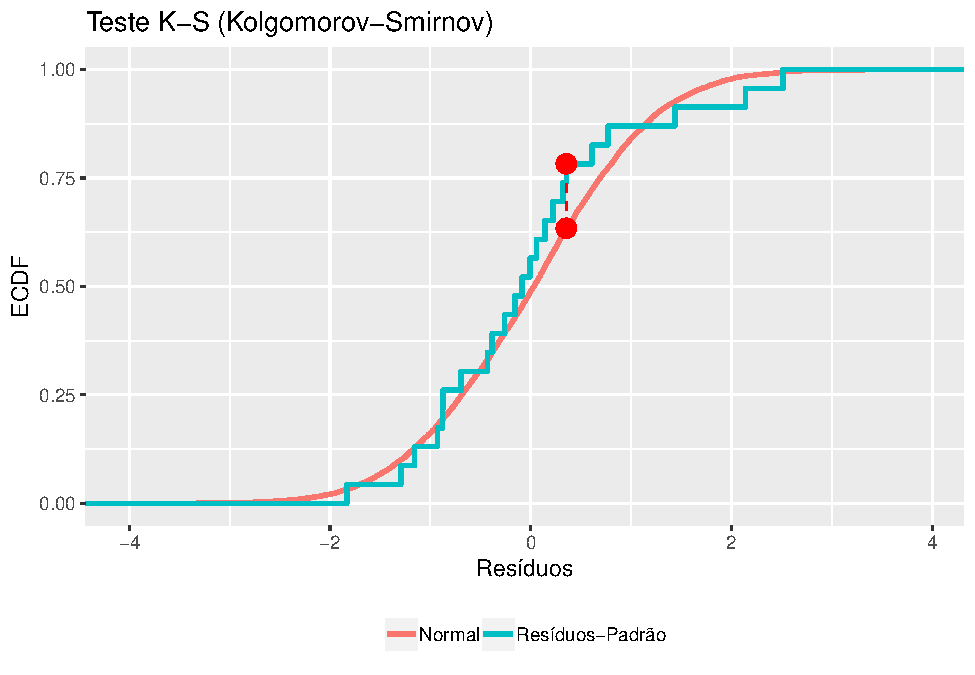
\includegraphics[width=0.45\linewidth]{Report_files/figure-latex/KS-1} 

}

\caption{Curva da função de distribuição acumulada (FDA) empírica}\label{fig:KS}
\end{figure}

\newpage

\subsubsection{Gráficos do modelo}\label{graficos-do-modelo}

\begin{enumerate}
\def\labelenumi{\alph{enumi}.}
\tightlist
\item
  Na mediana das variáveis
\end{enumerate}

\begin{figure}[H]

{\centering 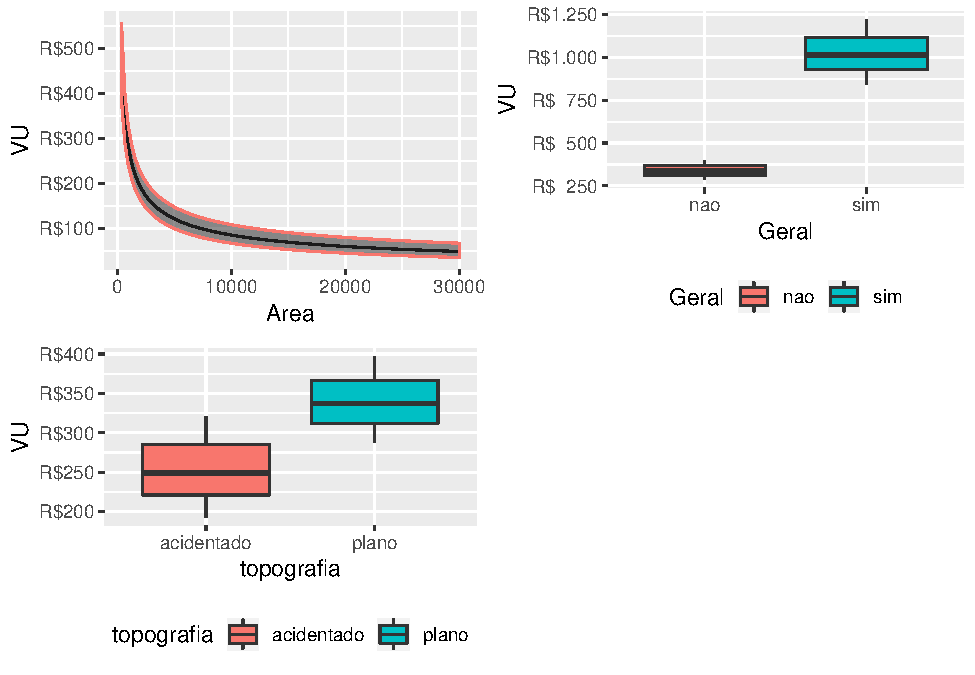
\includegraphics[width=1\linewidth]{Report_files/figure-latex/unnamed-chunk-8-1} 

}

\caption{Gráficos dos regressores em função da variável dependente (em cada gráfico, os outros regressores estão em seus valores médios.}\label{fig:unnamed-chunk-8}
\end{figure}

\newpage

\begin{enumerate}
\def\labelenumi{\alph{enumi}.}
\setcounter{enumi}{1}
\tightlist
\item
  No ponto de avaliação
\end{enumerate}

\begin{figure}[H]

{\centering 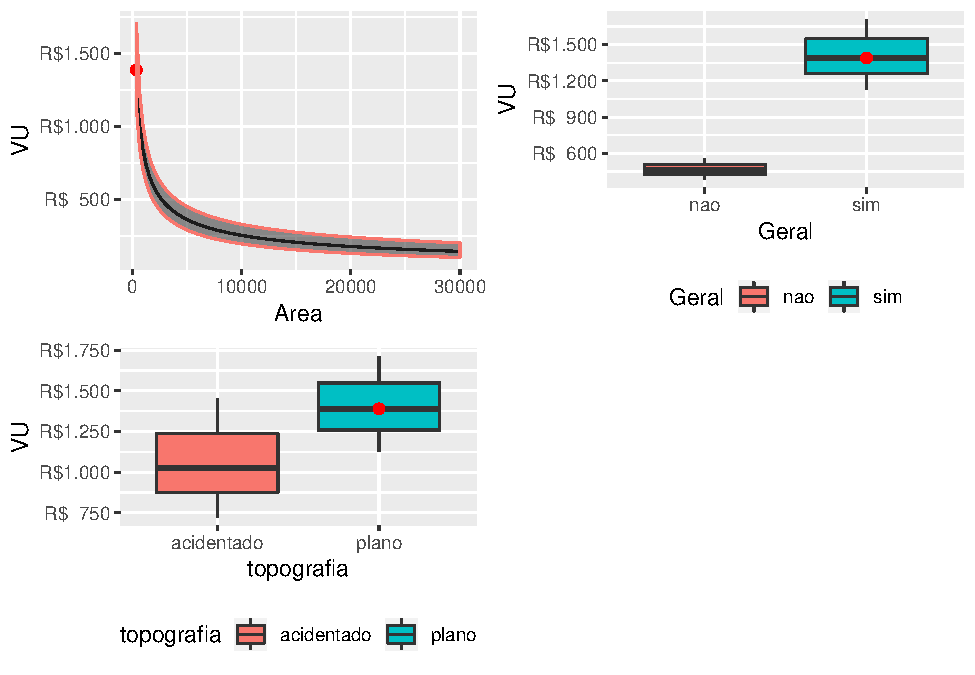
\includegraphics[width=1\linewidth]{Report_files/figure-latex/unnamed-chunk-9-1} 

}

\caption{Gráficos dos regressores em função da variável dependente (em cada gráfico, os outros regressores estão com os valores reais do avaliando.}\label{fig:unnamed-chunk-9}
\end{figure}

\newpage

\begin{enumerate}
\def\labelenumi{\Roman{enumi}.}
\setcounter{enumi}{3}
\tightlist
\item
  Poder de Predição
\end{enumerate}

\begin{figure}[H]

{\centering 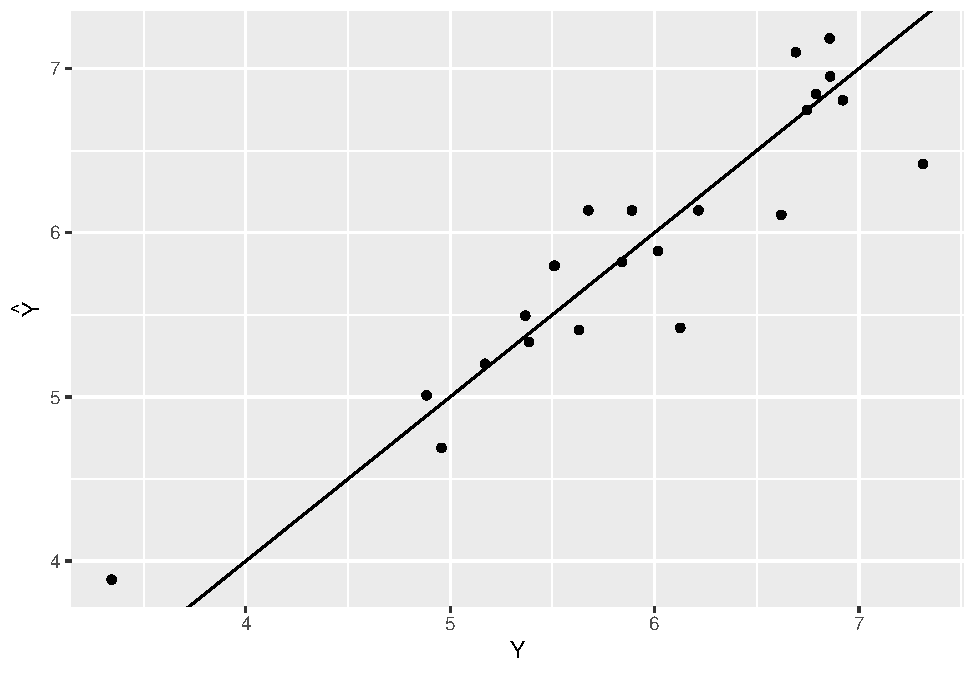
\includegraphics[width=0.5\linewidth]{Report_files/figure-latex/unnamed-chunk-10-1} 

}

\caption{Poder de Predição.}\label{fig:unnamed-chunk-10}
\end{figure}


\end{document}
